%%%%%%%%%%%%%%%%%%%%%%%%%%%%%%%%%%%%%%%%%
% FRI Data Science_report LaTeX Template
% Version 1.0 (28/1/2020)
% 
% Jure Demšar (jure.demsar@fri.uni-lj.si)
%
% Based on MicromouseSymp article template by:
% Mathias Legrand (legrand.mathias@gmail.com) 
% With extensive modifications by:
% Antonio Valente (antonio.luis.valente@gmail.com)
%
% License:
% CC BY-NC-SA 3.0 (http://creativecommons.org/licenses/by-nc-sa/3.0/)
%
%%%%%%%%%%%%%%%%%%%%%%%%%%%%%%%%%%%%%%%%%


%----------------------------------------------------------------------------------------
%	PACKAGES AND OTHER DOCUMENT CONFIGURATIONS
%----------------------------------------------------------------------------------------
\documentclass[fleqn,moreauthors,10pt]{ds_report}
\usepackage[english]{babel}

% https://tex.stackexchange.com/questions/89115/how-to-rotate-text-in-multirow-table
\usepackage{multirow}
\newcommand{\STAB}[1]{\begin{tabular}{@{}c@{}}#1\end{tabular}}
\usepackage{tabularx}

\graphicspath{{fig/}}




%----------------------------------------------------------------------------------------
%	ARTICLE INFORMATION
%----------------------------------------------------------------------------------------

% Header
\JournalInfo{FRI Data Science Project Competition 2023}

% Interim or final report
%\Archive{Interim report} 
\Archive{Final report} 

% Article title
\PaperTitle{Question answering pipeline for closed domain questions} 

% Authors (student competitors) and their info
\Authors{Luka \v{S}kodnik and Robert Jutre\v{s}a}

% Advisors
\affiliation{\textit{Advisors: prof. dr. Marko Robnik Šikonja, Grega Jerkič, dr. Branislava Šandrih Todorović}}

% Keywords
\Keywords{question answering, large language models, financial domain}
\newcommand{\keywordname}{Keywords}


%----------------------------------------------------------------------------------------
%	ABSTRACT
%----------------------------------------------------------------------------------------

\Abstract{
For this project, we are tasked with experimenting with possible implementations of closed-domain question-answering systems for the NLB Group. To this end we use large language models, focusing on two approaches: text extraction and text generation. In addition to this, a relevant context (one containing an answer) has to be passed into the models. To select one we employ a dense passage retrieval model together with a relevant document store. In order to find the optimal method, we fine-tune all of the components on the available data. The achieved results provide a good baseline, for further improvements and developments, using additional expert data and larger models.
}
% In this project, we use large language models for question answering, focusing on two approaches: extractive and generative. In the extractive approach, the span of the answer within the context is extracted, while in the generative approach, the answer is generated based on the given question and relevant context. The choice of a relevant context from a document or a set of documents is crucial for the performance of the system, and a separate retriever is typically used to select the most informative contexts. Extractive models perform well when the answer is a substring of the context, while generative models can handle more complex questions and reasoning on the context. We plan to implement both approaches and compare their performance.
%\textbf{TODO: update}

%----------------------------------------------------------------------------------------

\begin{document}

% Makes all text pages the same height
\flushbottom

% Print the title and abstract box
\maketitle
% Removes page numbering from the first page
\thispagestyle{empty}

%----------------------------------------------------------------------------------------
%	ARTICLE CONTENTS
%----------------------------------------------------------------------------------------

\section*{Introduction}
	%In the Introduction section you should write about the relevance of your work (what is the purpose of the project, what will we solve) and about related work (what solutions for the problem already exist). Where appropriate, reference scientific work conducted by other researchers. For example, the work done by Demšar et al. \cite{Demsar2016BalancedMixture} is very important for our project. The abbreviation et al. is for et alia, which in latin means and others, we use this abbreviation when there are more than two authors of the work we are citing. If there are two authors (or if there is a single author) we just write down their surnames. For example, the work done by Demšar and Lebar Bajec \cite{Demsar2017LinguisticEvolution} is also important for successful completion of our project.


    In the past years, the quality of Natural Language Processing (NLP) tools that use Large Language Models (LLM) drastically increased.
    This prompted a large number of companies to start introducing them into their work environment in order to cut down on employees' time and increase productivity.
    To this end, we adapt existing models and approaches for open domain question answering (QA) to our specific domain - banking.
    Using various techniques, we implement and evaluate different question-answering pipelines, by fine-tuning open-source models with domain-specific data that has been provided to us. \\
    In this paper, we first outline the state-of-the-art datasets and models for the domain of question answering. We then present the data, models, and evaluation procedures used, giving an outline of the structure and behavior of the final model. Next, we show both the quantitative and qualitative results and comment on them briefly. Finally, we discuss what these results mean, how we could improve them, and what the conclusions of our experiments are.
    % FROM interim report - update
    % The goal is to build a production-ready model, that outperforms baseline approaches for the required tasks.
    


%------------------------------------------------
% added related work section - since this may not end up like a scientific paper maybe we should think about including this in some other chapter
\section*{Related Work}

\subsection*{Datasets}

The most widely used dataset for open-domain question answering is Stanford Question and Answering Dataset (SQuA\-D)~\cite{rajpurkar2016squad, rajpurkar2018squadv2}.
Originally containing over 100k questions with corresponding passages (contexts) and answers, it was later extended to also include over 50k questions without an answer, with the intention of improving models by ensuring more accurate learning when a context does not contain an answer.
TriviaQA~\cite{joshi2017triviaqa} and WikiQA~\cite{yang2015wikiqa} are also general question-answering datasets, that use the same data structure as SQuAD. We use that same data structure for our own dataset.
%, which we also used.
HotpotQA~\cite{yang2018hotpotqa} is a dataset that aims to mitigate some of the drawbacks of extractive models and the SuperGLUE~\cite{SuperGLUE} benchmark contains datasets for different language understanding tasks including question answering. 
It formulates question-answering tasks in multiple ways: yes/no questions, multiple choice questions, and queries where an answer is located at a certain position.

\subsection*{Models}
Question-answering tasks that are the most relevant to us include extractive QA and generative QA.
For extractive QA models, which extract the answer from a given context, the most widely used approach is to adapt the BERT~\cite{devlin2019bert} model on datasets such as SQuAD.
Generative models such as GPT~\cite{openai2023gpt4}, T5~\cite{T5}, LLaMA~\cite{touvron2023llama}, and BLOOM~\cite{scao2022bloom}, can also be trained to generate an answer to a question, either from a provided context or without a context whatsoever. \\
To obtain contexts from a larger text database from which to extract/generate an answer, many systems use Dense Passage Retrieval (DPR)~\cite{karpukhin2020dense}.
It uses question and context encoders and returns a paragraph with the highest relevance to the answer.


%------------------------------------------------
\section*{Methodology}
\subsection*{Data}
The data available to us were the annual sustainability reports of the NLB banking group.
These reports are publicly available and contain data about the development and working culture of the bank.
To implement a QA model, question-context-answer pairs have to be extracted from selected sources, and formatted to suit the already pre-trained models.
To achieve this, we used the pre-built QA generation pipeline from Haystack~\cite{haystack}.
This data was filtered by NLB banking experts, and post-processed to ensure standard formatting.
This process returned 185 questions from the 2020 yearly report and 355 from the 2022 report.
Later on, we received 62 expert question-context-answer pairs of higher quality.
All of these datasets are randomly split into train and test sets, using a 70-30 split. \\
In addition, we use a prebuilt script (provided by Haystack) to transform the question-context-answer pairs from the SQ\-uAD to the DPR format, which is used to fine-tune the DPR model.
% Half of the test set was then used for validation during fine-tuning.\\
% {\it Furthermore, we are expecting another set of question-answer pairs to be provided to us, written by the NLB banking experts. These will be processed and used at a later date. When this data is acquired, the data will then be joined an formally split into the train, validation and test sets.}
% \noindent\textbf{70-30 split, no validation (we have too little data?), 2020 and 2022 and hadwritten data}

\subsection*{Question answering pipeline}

\begin{figure}[hbt]\centering
	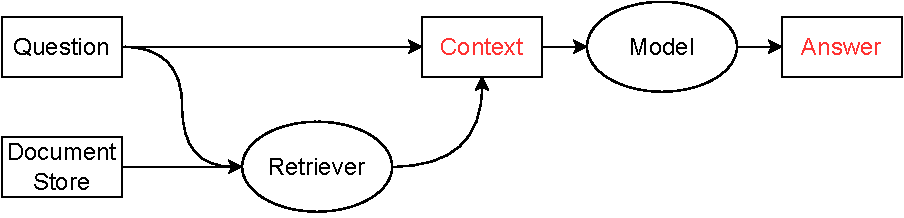
\includegraphics[width=0.9\linewidth]{fig/model_diagram.pdf}
	\caption{The diagram of our pipeline. Red denotes the output of the previous component.}
	\label{fig:pipeline}
\end{figure}

\noindent The outline of our pipeline can be observed in Figure~\ref{fig:pipeline} and its components are briefly described below. All used models are part of the HuggingFace library~\cite{wolf2019huggingface}.

\noindent We considered two approaches: extractive and generative.
In the extractive approach, models try to find the answer in a given context. This approach is reliable for more straightforward questions.
There are multiple limitations of this approach since models can accept only a limited length context and the answer might not always be contained in the context.
We explored two variants of BERT, called DistilBERT~\cite{sanh2019distilbert} and RoBERTa~\cite{liu2019roberta}, which have already been pre-trained on the SQuAD dataset.
% Our preliminary model was a smaller variant of BERT called DistilBERT~\cite{sanh2019distilbert} which has already been pre-trained on the SQuAD dataset.
% {\it Additional fine-tuning will have to be done after expanding the dataset. The full process will be explained here.}

\noindent Generative models learn to generate a sequence of words from the input query (and context if provided).
The benefit of these models is that they are able to answer more complex questions since they are not extracting the answer from the context but generating one based on language understanding and the provided context.
For this approach, we use the small and base version of the T5~\cite{T5} model which has been fine-tuned for question-answering on the SQuAD dataset.
% {\it This approach could be better suited for question-answer pairs that are written and not automatically generated, as we have no guarantee that the answer will be provided directly in the context, but may be paraphrased or expressed implicitly. The baseline models used for this approach will likely include T5 and LLaMA.}

\noindent Since both the extractive and generative models require contexts our pipeline has to provide one containing the answer.
A sliding window passing through all possible contexts would be computationally inefficient.
Therefore, we employ a context retriever model which identifies a small number of relevant contexts to the given question.
We employ the DPR~\cite{karpukhin2020dense} model which was shown to outperform traditional methods such as TF-IDF~\cite{jalilifard2021semantic} or BM25~\cite{robertson2009probabilistic}.
% {\it Here the DPR model will be used as the first part of the pipeline, to find and extract the required context, and its output will be fed to the QA model to return the answer.}

\noindent To leverage the additional information contained in the provided data, we fine-tune all the components on the available data.
We test multiple combinations of the components, choosing between the extractive or generative model and different data used to fine-tune those models.

\subsection*{Evaluation metrics}
For evaluation, we consider several metrics. Since SQuAD has its own evaluation benchmark, this is our first choice. 
The second metric, BLEU~\cite{papineni2002bleu}, is a benchmark for evaluating translation models. Here we use it to match the returned answer with the ground truth (GT).
Lastly, we use Bertscore~\cite{zhang2019bertscore}, which returns the precision, recall, and F1 score between the returned answer and the GT.
% {\it Based on our dataset, we will also consider the SuperGLUE ReCoRD and MultiRC tasks in our evaluation.}

%------------------------------------------------
\section*{Results}

\subsection*{Model performance}
\begin{table}[hbt]
	\caption{Extractive model performance. \textit{Fine} refers to the fine-tuned model.}
	\centering
    \label{tab:bert_fine_tuning}
    \scalebox{0.7}{
    	\begin{tabular}{c l || c c c | c | c c}
    		  & & \multicolumn{3}{c|}{Bertscore} & Bleu & \multicolumn{2}{c}{SQuAD}\\
    		& Model                & Precision & Recall & F1 & & Exact & F1 \\
            \hline \hline
            \multirow{4}{*}{\STAB{\rotatebox[origin=c]{90}{20/22}}}
            & distil               & $85.94$ & $92.17$ & $87.49$ & $9.22$  & $37.32$ & $48.68$ \\
            & distil-fine          & $88.13$ & $92.54$ & $89.52$ & $11.69$ & $38.73$ & $50.50$ \\
            \cmidrule(lr){2-8}
            & roberta              & $70.46$ & $91.12$ & $71.78$ & $26.46$ & $38.03$ & $46.47$ \\
            & roberta-fine         & $\textbf{89.07}$ & $\textbf{93.64}$ & $\textbf{90.76}$ & $\textbf{32.09}$ & $\textbf{47.18}$ & $\textbf{59.32}$ \\
            \hline \hline
            \multirow{4}{*}{\STAB{\rotatebox[origin=c]{90}{expert}}}
            & distil               & $\textbf{87.71}$ & $86.50$ & $87.04$ & $15.36$ & $\textbf{15.79}$ & $37.71$ \\
            & distil-fine          & $87.68$ & $\textbf{88.28}$ & $\textbf{87.90}$ & $37.81$ & $10.53$ & $45.52$ \\
            \cmidrule(lr){2-8}
            & roberta              & $56.82$ & $82.55$ & $57.13$ & $0.53$  & $5.26$  & $22.14$ \\
            & roberta-fine         & $75.83$ & $87.73$ & $79.33$ & $\textbf{47.66}$ & $\textbf{15.79}$ & $\textbf{47.09}$
            
    	\end{tabular}
     }
\end{table}

\begin{table}[hbt]
	\caption{Generative model performance. \textit{Fine} refers to the fine-tuned model.}
	\centering
    \label{tab:t5_fine_tuning}
    \scalebox{0.7}{
    	\begin{tabular}{c l || c c c | c }
    		  & & \multicolumn{3}{c|}{Bertscore} & Bleu \\
            & Model              & Precision & Recall & F1 & \\
            \hline \hline
            \multirow{4}{*}{\STAB{\rotatebox[origin=c]{90}{20/22}}}
            & t5-small                & $95.07$ & $95.54$ & $95.28$ & $55.46$ \\
            & t5-small-fine      & $97.03$ & $98.16$ & $97.57$ & $54.31$ \\
            \cmidrule(lr){2-6}
            & t5-base                 & $88.29$ & $90.95$ & $89.55$ & $12.71$ \\
            & t5-base-fine       & $\textbf{98.07}$ & $\textbf{98.44}$ & $\textbf{98.25}$ & $\textbf{68.27}$ \\
            \hline \hline
            \multirow{4}{*}{\STAB{\rotatebox[origin=c]{90}{expert}}}
            & t5-small                & $89.48$ & $86.39$ & $87.87$ & $6.74$ \\
            & t5-small-fine      & $92.26$ & $88.93$ & $90.52$ & $22.11$ \\
            \cmidrule(lr){2-6}
            & t5-base                 & $83.70$ & $84.70$ & $84.13$ & $12.81$ \\
            & t5-base-fine       & $\textbf{93.21}$ & $\textbf{92.25}$ & $\textbf{92.68}$ & $\textbf{52.30}$
            
    	\end{tabular}
     }
\end{table}

\noindent In Table~\ref{tab:bert_fine_tuning} and Table~\ref{tab:t5_fine_tuning} we can observe the results obtained by the extractive and generative models before and after additional fine-tuning.
We fine-tuned the models on the train splits of automatically generated data from 2020, 2022, and combined 20/22, as well as on the expert data.

\noindent We observe that fine-tuning a model results in better metrics in most cases.
On the automatically generated data, we get good results without additional fine-tuning and observe a similar increase after fine-tuning, regardless of the dataset. 
When evaluating on only a specific year, rather than the combined data, we do see better performance for the respectfully fine-tuned models. However, we deem the combined data more important and thus exclude others from the tables for the sake of brevity.

\noindent The biggest difference in performance is observed with the expert data, where the increase is large, especially for the BLEU score. Many models don't gain a significant increase in performance after fine-tuning.
This was expected since the automatically generated data resembles the data in SQuAD much more than the expert data.
For this reason, the information gained was smaller in contrast to fine-tuning on the expert data, which is more distinct.

\noindent Using the automatically generated data we tried fine-tuning the models on only half of the train set to see if training on less data impacts the performance significantly.
Albeit worse, the metrics, for models fine-tuned this way, are close enough to question whether the additional work required (filtering all of the automatically generated data) is worth the slight increase in performance.

\begin{table}[hbt]
	\caption{Mean and standard deviation scores for the T5-small model over 10 different train/test splits.}
	\centering
    \label{tab:uncertainty}
    \scalebox{0.65}{
    	\begin{tabular}{c l || c c c | c }
    		  & & \multicolumn{3}{c|}{Bertscore} & Bleu \\
            & & Precision & Recall & F1 & \\
            \hline \hline
            \multirow{2}{*}{\STAB{\rotatebox[origin=c]{90}{20/22}}}
            % & & & & &\\
            & mean                & $96.98$ & $97.78$ & $97.35$ & $57.73$ \\
            & std                 & $0.35$ & $0.34$ & $0.33$ & $3.25$ \\
            % & & & & &\\
            \hline \hline
            \multirow{2}{*}{\STAB{\rotatebox[origin=c]{90}{expert}}}
            % & & & & &\\
            & mean                & $91.79$ & $88.48$ & $90.06$ & $19.65$ \\
            & std                 & $1.17$ & $1.16$ & $1.22$ & $7.04$ \\
            % & & & & &\\
            
    	\end{tabular}
     }
\end{table}

\noindent We decided to check the uncertainty of the dataset by training the same model 10 times with a different 70-30 train/test split on both the combined and expert datasets. The results of this can be seen in Table~\ref{tab:uncertainty}. We expected the standard deviation to be higher for the expert data set as there are not a lot of questions and they differ quite substantially, and this is indeed the case. Meanwhile, the standard deviation for the generated data is lower, due to the fact that we have a lot more (similar) data in that set.

%%%%%%%%%%%%%%%%%%
\subsection*{Pipeline performance}

\begin{table}[hbt]
	\caption{Pipeline performance using fine-tuned models. }
	\centering
    \label{tab:pipeline}
    \scalebox{0.65}{
    	\begin{tabular}{c c l || c c c | c | c c}
    		  & & & \multicolumn{3}{c|}{Bertscore} & Bleu & \multicolumn{2}{c}{SQuAD}\\
    		& & Model                & Precision & Recall & F1 & & Exact match & F1 \\
            \hline \hline
            \multirow{8}{*}{\STAB{\rotatebox[origin=c]{90}{20/22}}}
            & \multirow{4}{*}{\STAB{\rotatebox[origin=c]{90}{DPR}}}
            &  distil-fine   & $91.75$ & $91.41$ & $91.57$ & $12.22$ & $23.94$ & $27.64$ \\
            && roberta-fine  & $\textbf{92.85}$ & $\textbf{92.84}$ & $\textbf{92.83}$ & $\textbf{29.09}$ & $\textbf{35.21}$ & $\textbf{37.89}$ \\
            && t5-small-fine & $92.18$ & $92.50$ & $92.33$ & $15.24$ & / & / \\
            && t5-base-fine  & $91.64$ & $92.02$ & $91.81$ & $16.79$ & / & / \\
            \cmidrule(lr){2-9}
            & \multirow{4}{*}{\STAB{\rotatebox[origin=c]{90}{DPR-fine}}}
    		&  distil-fine   & $91.88$ & $91.61$ & $91.73$ & $15.18$ & $27.46$ & $31.70$ \\
            && roberta-fine  & $\textbf{93.18}$ & $\textbf{93.03}$ & $\textbf{93.09}$ & $\textbf{33.23}$ & $\textbf{36.62}$ & $\textbf{39.93}$ \\
            && t5-small-fine  & $91.94$ & $92.68$ & $92.04$ & $14.53$ & / & / \\
            && t5-base-fine & $92.06$ & $92.49$ & $92.25$ & $18.28$ & / & / \\
            \hline \hline
            \multirow{8}{*}{\STAB{\rotatebox[origin=c]{90}{expert}}}
            & \multirow{4}{*}{\STAB{\rotatebox[origin=c]{90}{DPR}}}
            &  distil-fine   & $86.98$ & $86.94$ & $86.93$ & $0.0$   & $\textbf{4.76}$ & $11.58$ \\
            && roberta-fine  & $88.15$ & $87.33$ & $87.63$ & $4.61$  & $\textbf{4.76}$ & $\textbf{21.53}$ \\
            && t5-small-fine & $\textbf{88.78}$ & $87.44$ & $\textbf{88.04}$ & $13.48$ & / & / \\
            && t5-base-fine  & $86.11$ & $\textbf{88.20}$ & $87.06$ & $\textbf{24.60}$ & / & / \\
            \cmidrule(lr){2-9}
            & \multirow{4}{*}{\STAB{\rotatebox[origin=c]{90}{DPR-fine}}}
    		&  distil-fine   & $87.41$ & $87.19$ & $87.25$ & $0.0$ & $4.76$ & $16.87$ \\
            && roberta-fine  & $\textbf{88.78}$ & $\textbf{87.75}$ & $\textbf{88.21}$ & $5.10$ & $\textbf{14.29}$ & $\textbf{27.57}$ \\
            && t5-small-fine & $86.92$ & $85.23$ & $86.03$ & $0.88$ & / & / \\
            && t5-base-fine  & $85.45$ & $87.42$ & $86.38$ & $\textbf{18.75}$ & / & / \\
        
    	\end{tabular}
     }
\end{table}

\noindent In Table~\ref{tab:pipeline} we can observe the results obtained using fine-tuned models in combination with a DPR that has or hasn't been fine-tuned (on automatically generated data).
The DPR retrieves the contexts from both the reports for the combined 20/22 data or only from the 2022 report for the expert data. 
We can see that fine-tuning the DPR has a positive effect as a higher number of exact matches are achieved (alongside an increase in other metrics).
This means that the DPR managed to retrieve more relevant contexts and the models can provide better answers.
% The exception to this are the generative models fine-tuned on expert data using a fine-tuned DPR.

\subsection*{Qualitative analysis}

\begin{table}[hbt]
	\caption{Qualitative analysis of the QA pipeline on combined and expert data}
	\centering
    \label{tab:pipeline_qualitative}
    \scalebox{0.65}{
    	\begin{tabular}{c l || c c c l | c c c l | c}
    		&       & \multicolumn{4}{c|}{Correctness} & \multicolumn{4}{c|}{Sensibility} & ``None`` \\
            & Model & $1$ & $2$ & $3$ & avg [\%] & $1$ & $2$ & $3$ & avg [\%] & \\
            \hline \hline
            \multirow{4}{*}{\STAB{\rotatebox[origin=c]{90}{20/22}}}
            & distilbert    & $13$ & $1$ & $7$ & $\textbf{57}$ & $7$ & $5$ & $9$ & $\textbf{70}$ & $0$ \\
            & roberta       & $13$ & $1$ & $7$ & $\textbf{57}$ & $7$ & $5$ & $9$ & $\textbf{70}$ & $0$ \\
            & t5 small      & $13$ & $1$ & $7$ & $\textbf{57}$ & $7$ & $6$ & $8$ & $68.3$ & $0$ \\
            & t5 base       & $13$ & $1$ & $7$ & $\textbf{57}$ & $7$ & $5$ & $9$ & $\textbf{70}$ & $0$ \\
            \hline
            \multirow{4}{*}{\STAB{\rotatebox[origin=c]{90}{expert}}}
            & distilbert    & $17$ & $3$ & $1$ & $\textbf{41.3}$ & $8$ & $6$ & $7$ & $\textbf{65}$ & $0$ \\
            & roberta       & $18$ & $3$ & $0$ & $38$ & $11$ & $4$ & $6$ & $58.7$ & $0$ \\
            & t5 small      & $16$ & $5$ & $0$ & $\textbf{41.3}$ & $12$ & $3$ & $6$ & $57$ & $7$ \\
            & t5 base       & $17$ & $3$ & $1$ & $\textbf{41.3}$ & $14$ & $1$ & $6$ & $54$ & $0$ \\
    	\end{tabular}
     }
\end{table}

\begin{table*}[hbt]
% \footnotesize
\small
	\caption{Examples of retrieved contexts and obtained answers from the pipeline. An answer generated using ChatGPT is provided for comparison.}
 %In the first example the retreived context is ``correct`` and all the models answer correctly. In the second the retrieved context is relevant but not the one expected so we get a meaningful answer but different than the ground truth one. In the last example the retrieved context only mentions one thing in the question and does not contain any relevant information.}
	\centering
	\label{tab:examples}
    \scalebox{1}{
	\begin{tabular}{l}
        \hline \hline
        % 2042: 11
        % \textbf{Question}: How many Slovenian companies joined the GREENVISION initiative? \textbf{GT Answer}: almost 100\\
        \textbf{Question}: How many branches does NLB Group have in all markets where it operates? \textbf{GT Answer}: 440\\
        \textbf{Retreived context}: NLB Group in numbers (as at 31 December 2022)\\
        • An extensive network of 440 branches in all markets where NLB Group operates.\\
        • More than 2.7 million active customers.\\
        • With successful operations, NLB Group generated a record high profit of €446.9 million in 2022, with the acquisition \\ of N Banka in March significantly influencing the full-year business results of the Group.\\
        • The balance sheet total of the NLB Group amounts to €24.2 billion.\\
        \hline
		\textbf{Answers} $\mid$ distilbert: ``440`` $\mid$ roberta: ``440`` $\mid$ t5-small: ``440`` $\mid$ t5-base: ``440``\\
        \hline
        \textbf{ChatGPT Answer}: Based on the provided context, the number of branches NLB Group has in all markets where it operates is 440. \\
        \hline \hline
        % 2042: 5
        \textbf{Question}: How much did the bank reduce the use of paper in 2022 compared to the previous year? \textbf{GT Answer}: 19\%\\
        \textbf{Retreived context}: In 2022, another step to achieving this goal has been made as paper usage (prints) was reduced \\
        by 17\% compared to 2021. Thus, we saved 866 trees. Paper usage in NLB was lower by 26\%, which is the highest\\
        reduction group – wide. All banking subsidiaries experienced reduction as well, ranging from 8\% to 19\%, respectively.\\
        \hline
		\textbf{Answers} $\mid$ distilbert: ``17\%`` $\mid$ roberta: ``17\%`` $\mid$ t5-small: ``17\%`` $\mid$ t5-base: ``17\%``\\
        \hline
        \textbf{ChatGPT Answer}: Based on the given context, the bank reduced the use of paper by 17\% compared to the previous year\\
        (2021). However, the exact amount of paper usage in 2021 or any specific quantity of paper used is not mentioned.\\
        \hline \hline
        % expert 13
        %\textbf{Question}: How much new green loan NLB Group generated for retail clients? \textbf{GT Answer}: Over €53 million\\
        %\textbf{Retreived context}: NLB Green Housing loan (SDG 11,12,13) Purposes: for purchasing or building a passive house, for\\
        %purchase and installation of solar power plants with or w/o battery, for heat pumps, charging stations, IR panels, and gas\\
        %boilers 2. NLB Green partner loan (SDG 11, 12,13) Purposes: for purchase and installation of solar power plants with or\\
        %w/o battery, for heat pumps, charging stations, IR panels, and gas boilers NLB Group finances corporate clients for\\
        %projects such as: • wind farms, • solar power plants, • energy-efficient buildings. ››› 1. For more information\\
        %about client engagement, please refer to: Sustainability Report 2022 p. 12 ››› 2. \\
        %hline
		%\textbf{Answers} $\mid$ distilbert: ``13`` $\mid$ roberta: ``›››`` $\mid$ t5-small: ``None`` $\mid$ t5-base: ``NLB Green partner loan (SDG 11, 12,13)``\\
        %\hline
        %\textbf{ChatGPT Answer}: The context provided does not mention the specific amount of new green loans generated by NLB Group\\
        %for retail clients. It only outlines the types of green loans offered by NLB Group, such as the NLB Green Housing loan and NLB\\
        %Green partner loan, along with their purposes.\\
        %\hline \hline
        
	\end{tabular}
    }
\end{table*}

\noindent To better gauge how well the pipeline works we look through the entire test set (21 examples) of expert questions and a subset of the automatically generated questions (21 examples that were selected arbitrarily).
We score the answers based on sensibility - how closely the retrieved context matches the topic of the question, and correctness - how close is the obtained answer to the GT.
We assign a number from 1 (worst) to 3 (best) for each example and mark the number of questions for which we get no answer - the model thinks it cannot answer the question from the provided context.

\noindent We can observe the results in Table \ref{tab:pipeline_qualitative}.
The results are quite poor since a lot of the time the ``wrong`` context is retrieved.
Sensibility always scores better than correctness since the context usually contains some information that is related to the question. The answer, however, still might not be considered correct, since the returned answer doesn't match the GT.
We observe that the more straightforward questions from the automatically generated data yield better results than the expert ones.
This is not surprising as some of the expert questions are fairly long and complex.
From the model and pipeline evaluation, we expected better performance from the generative models at least in the case of the more complex (expert) data.
The scores do not indicate this without looking at the number of times that we get the answer ``None``.
The small variant of T5 is the only model to correctly identify that the retrieved context does not contain the answer. It does this for 7 of the 21 selected examples.

\noindent In Table \ref{tab:examples} we can see 2 examples of retrieved contexts and the obtained answers.
When the context contains the GT answer we obtain the correct answer (1st example).
We also noticed two situations. Either the retrieved context contains a slightly different answer than the GT, which still could be considered correct (2nd example), or the retrieved context is irrelevant and all of the QA models fail.
We also include the answers obtained from a significantly larger model (ChatGPT) for comparison. As expected the use of a larger model yields much better results. However, in the case of the second example, this one also ``fails``.

%Use the results section to present the final results of your work. Present the results in a objective and scientific fashion. Use visualisations to convey your results in a clear and efficient manner. When comparing results between various techniques use appropriate statistical methodology.

%\subsection*{More random text}

%This text is inserted only to make this template look more like a proper report. Lorem ipsum dolor sit amet, consectetur adipiscing elit. Etiam blandit dictum facilisis. Lorem ipsum dolor sit amet, consectetur adipiscing elit. Interdum et malesuada fames ac ante ipsum primis in faucibus. Etiam convallis tellus velit, quis ornare ipsum aliquam id. Maecenas tempus mauris sit amet libero elementum eleifend. Nulla nunc orci, consectetur non consequat ac, consequat non nisl. Aenean vitae dui nec ex fringilla malesuada. Proin elit libero, faucibus eget neque quis, condimentum laoreet urna. Etiam at nunc quis felis pulvinar dignissim. Phasellus turpis turpis, vestibulum eget imperdiet in, molestie eget neque. Curabitur quis ante sed nunc varius dictum non quis nisl. Donec nec lobortis velit. Ut cursus, libero efficitur dictum imperdiet, odio mi fermentum dui, id vulputate metus velit sit amet risus. Nulla vel volutpat elit. Mauris ex erat, pulvinar ac accumsan sit amet, ultrices sit amet turpis.

%Phasellus in ligula nunc. Vivamus sem lorem, malesuada sed pretium quis, varius convallis lectus. Quisque in risus nec lectus lobortis gravida non a sem. Quisque et vestibulum sem, vel mollis dolor. Nullam ante ex, scelerisque ac efficitur vel, rhoncus quis lectus. Pellentesque scelerisque efficitur purus in faucibus. Maecenas vestibulum vulputate nisl sed vestibulum. Nullam varius turpis in hendrerit posuere.

%Nulla rhoncus tortor eget ipsum commodo lacinia sit amet eu urna. Cras maximus leo mauris, ac congue eros sollicitudin ac. Integer vel erat varius, scelerisque orci eu, tristique purus. Proin id leo quis ante pharetra suscipit et non magna. Morbi in volutpat erat. Vivamus sit amet libero eu lacus pulvinar pharetra sed at felis. Vivamus non nibh a orci viverra rhoncus sit amet ullamcorper sem. Ut nec tempor dui. Aliquam convallis vitae nisi ac volutpat. Nam accumsan, erat eget faucibus commodo, ligula dui cursus nisi, at laoreet odio augue id eros. Curabitur quis tellus eget nunc ornare auctor.


%------------------------------------------------

\section*{Discussion}
% Thus far, we have identified the main approaches for solving our problem and defined the pipeline.
% We started by fine tuning a model for the extractive approach and shown that fine tuning on our domain specific data improves the performance of the model.
% When we receive the data written by the banking experts we plan on using that data to fine tune our models as it should be of better quality.
% Knowing that this approach works we plan on adapting a context retriever to extract the relevant contexts from the annual reports.
% After this, we plan to fine tune additional model(s) for the extractive approach and test the generative approach.
% Finally, we plan to identifying more realistic evaluation protocols including human evaluation where we would manually check a sample of the answers generated by the models.

\noindent We consider two important factors when drawing conclusions from obtained results. These factors are the data and the models as well as the pipeline. We believe that each of these two factors plays an important role and making alterations to each of them could improve the performance.

\noindent First let's consider the data.
We were somewhat limited by the data available to us.
We haven't mentioned thus far that over 4000 question-context-answer pairs were generated.
These were filtered by the NLB banking professionals, to only include those that would be useful to them.
The remaining 540 pairs, together with the expert examples, provide a good starting point to fine-tune the models.
However, better results could be achieved with more data. This especially seems to be the case with the DPR model.
It was noticed during qualitative analysis that the pipeline is bottle-necked by its first component, and additional fine-tuning could alleviate this.
Better results could be achieved by using more expert data. As stated previously, the improvements seen when fine-tuning using expert data are the largest. Having more data of this type could increase the performance beyond the results reported here.
This wouldn't only allow us to answer more complex questions, but also achieve better results with smaller models. Better results could be possible, if we focused on a specific type of questions, for example, yes/no or multiple choice questions.

\noindent As already mentioned, to improve the pipeline we need to improve the DPR.
Another possible method to achieve this would be to modify the pipeline to use more than one context from the retriever to obtain one that actually has the answer.
On the other hand, the pipeline could also be improved by trying different models, e.g. ones with a longer context.
Implementing some Long Form Question-Answering (LFQA)~\cite{faneli5} models could possibly yield better results, as these can both accept longer questions and process much longer contexts.
Another improvement would be to use larger models.
As we noticed, ChatGPT outperforms our fine-tuned models, thus we can expect that using it, LLaMA, LaMDA~\cite{thoppilan2022lamda} or BART~\cite{lewis2019bart} in our pipeline would yield better results.
This would, however, require more computational power.

\noindent During the qualitative analysis we observe discrepancies with the quantitative results. The first reason is that the quantitative metrics can fail in some cases. For example, it has been studied that Bertscore fails when evaluating wrong answers with high lexical overlap~\cite{hanna2021fine}. The second reason is that qualitative analysis is in itself a biased and subjective process.
We assign much higher scores even if only one part of the pipeline works well which can't be easily included when obtaining the quantitative results.

\noindent Despite this we believe that the models do have their usefulness. The results show that they are good at answering more straightforward answers, most commonly those with a numeric answer. However, we don't deem these models production ready. We assume the models would require further fine-tuning with additional data or we could adapt larger models. With the currently available results, we conclude that the best cost-to-performance model is the small variant of T5. While the base variant and RoBERTa outperformed it in some metrics, it is the only model that correctly identifies when the answer isn't contained in the context.


%Use the Discussion section to objectively evaluate your work, do not just put praise on everything you did, be critical and exposes flaws and weaknesses of your solution. You can also explain what you would do differently if you would be able to start again and what upgrades could be done on the project in the future.


%------------------------------------------------

\section*{Acknowledgments}
We would like to thank our faculty advisor prof. dr. Marko Robnik Šikonja for providing irreplaceable guidance and advice. We would also like to thank dr. Branislava Sandrih Todorović and the NLB group for their cooperation, and our industry advisor Grega Jerkič for helping set the correct path and foundations of our work.

%Here you can thank other persons (advisors, colleagues ...) that contributed to the successful completion of your project.


% \cleardoublepage
\clearpage
%----------------------------------------------------------------------------------------
%	REFERENCE LIST
%----------------------------------------------------------------------------------------
\bibliographystyle{unsrt}
\bibliography{report}

\end{document}